\newpage

\section*{Anhang}
  \addcontentsline{toc}
    {section}
    {Anhang}



\subsection*{Elektronischer Anhang}\label{elect-anhang}
\addcontentsline{toc}
{subsection}
{Elektronischer Anhang}

Diese Dokumentation wurde zusammen mit einem elektronischen Anhang in Form einer ZIP-Datei abgegeben. Darin befinden sich der Simulator Programmiercode inklusive dessen Ergebnisse und die erstellten CAD Dateien.

\newpage
\subfile{parts/x-projektplanung}
\newpage

%%%%%%%%%%%%%%%%%% Aufgabenstellung

\subsection*{Originale Aufgabenstellung}\label{aufgabenstellung}
\addcontentsline{toc}
{subsection}
{Originale Aufgabenstellung}

Nachfolgend ist die originale Aufgabenstellung angehängt.

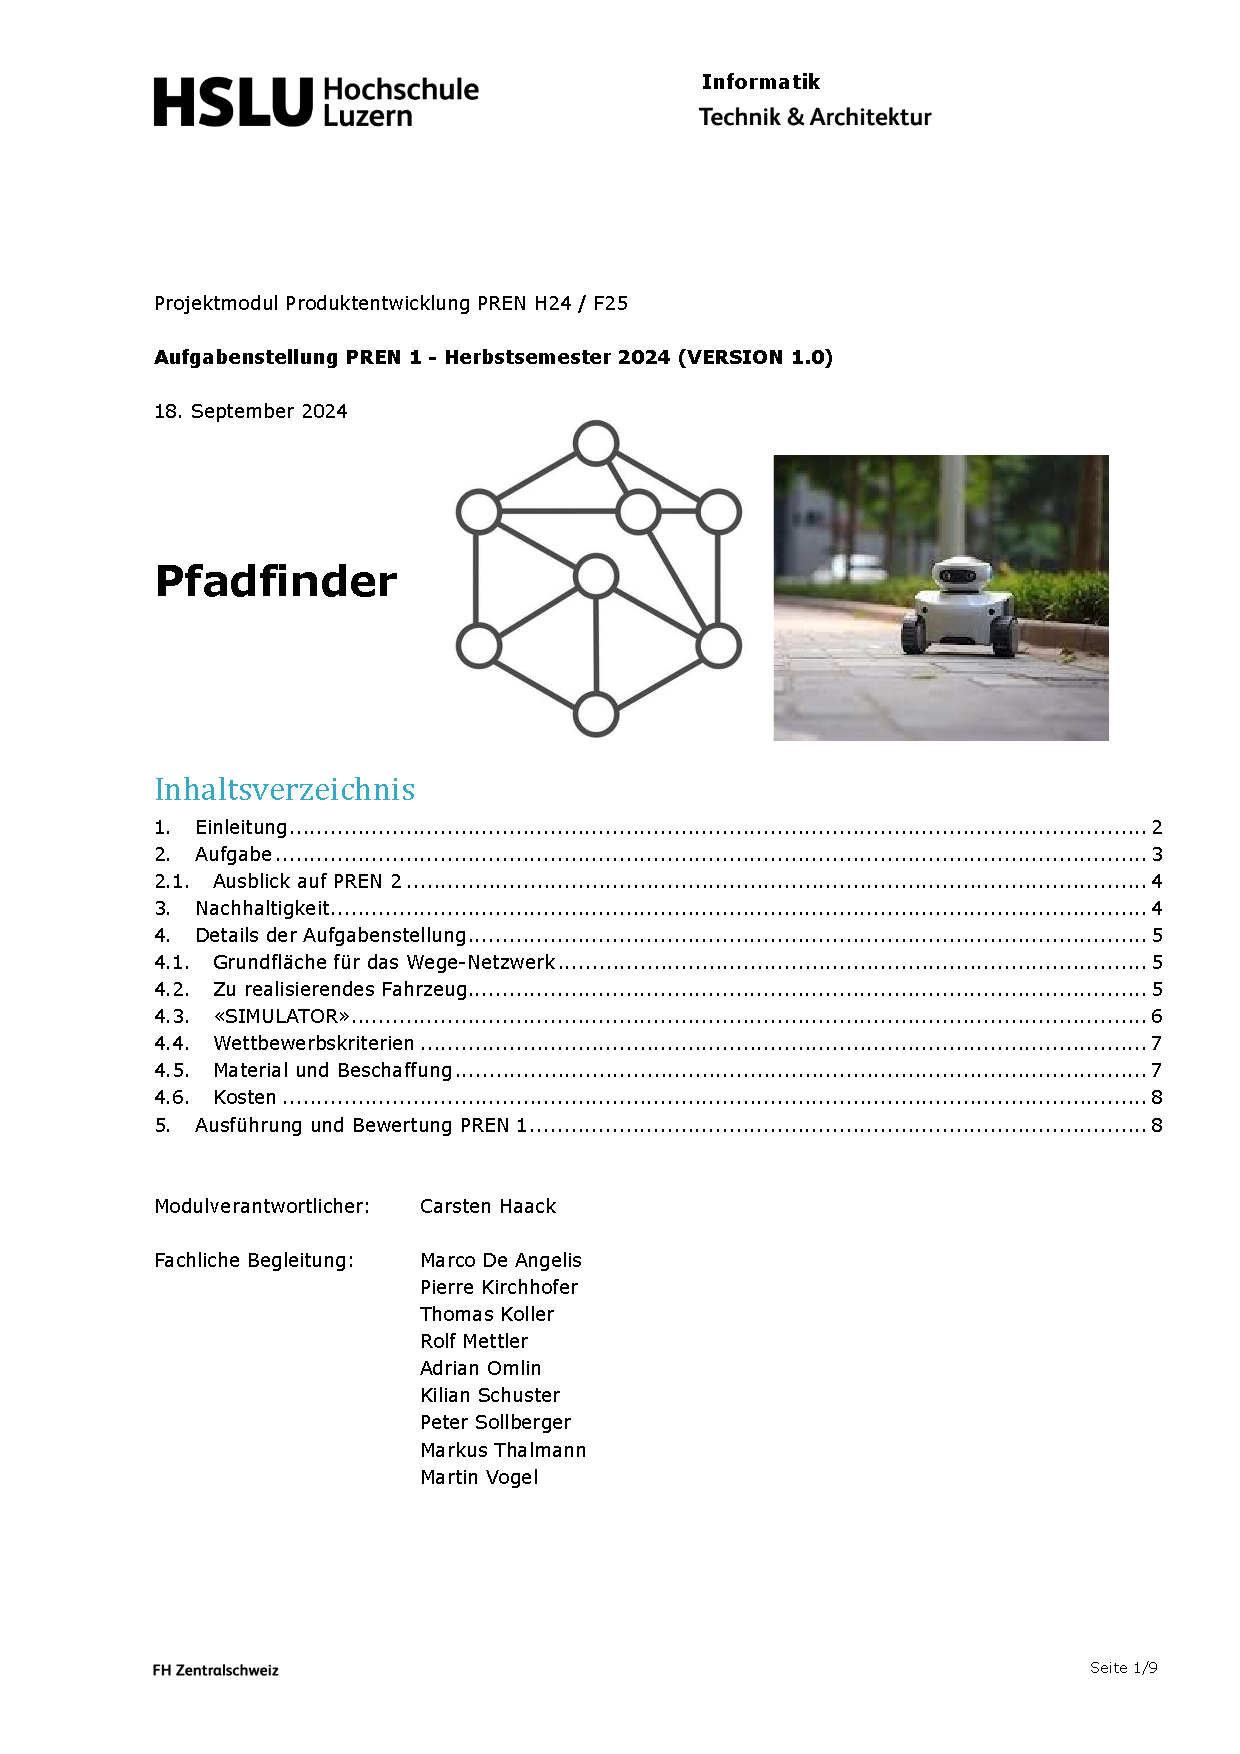
\includepdf[pages=-]{assets/projektmanagement/AufgabenstellungPREN1HS24.pdf}

%%%%%%%%%%%%%%% Anforderungsliste %%%%%%%%%%%%%%%%%%%%%%%%%

\subsection*{Anforderungsliste}\label{anforderungliste}
  \addcontentsline{toc}
    {subsection}
    {Anforderungsliste}
Die  Anforderungsliste ist ersichtlich in Tabellen \ref{table:anforderungsliste_page1} und \ref{table:anforderungsliste_page2}.

\begin{table}[H]
\centering
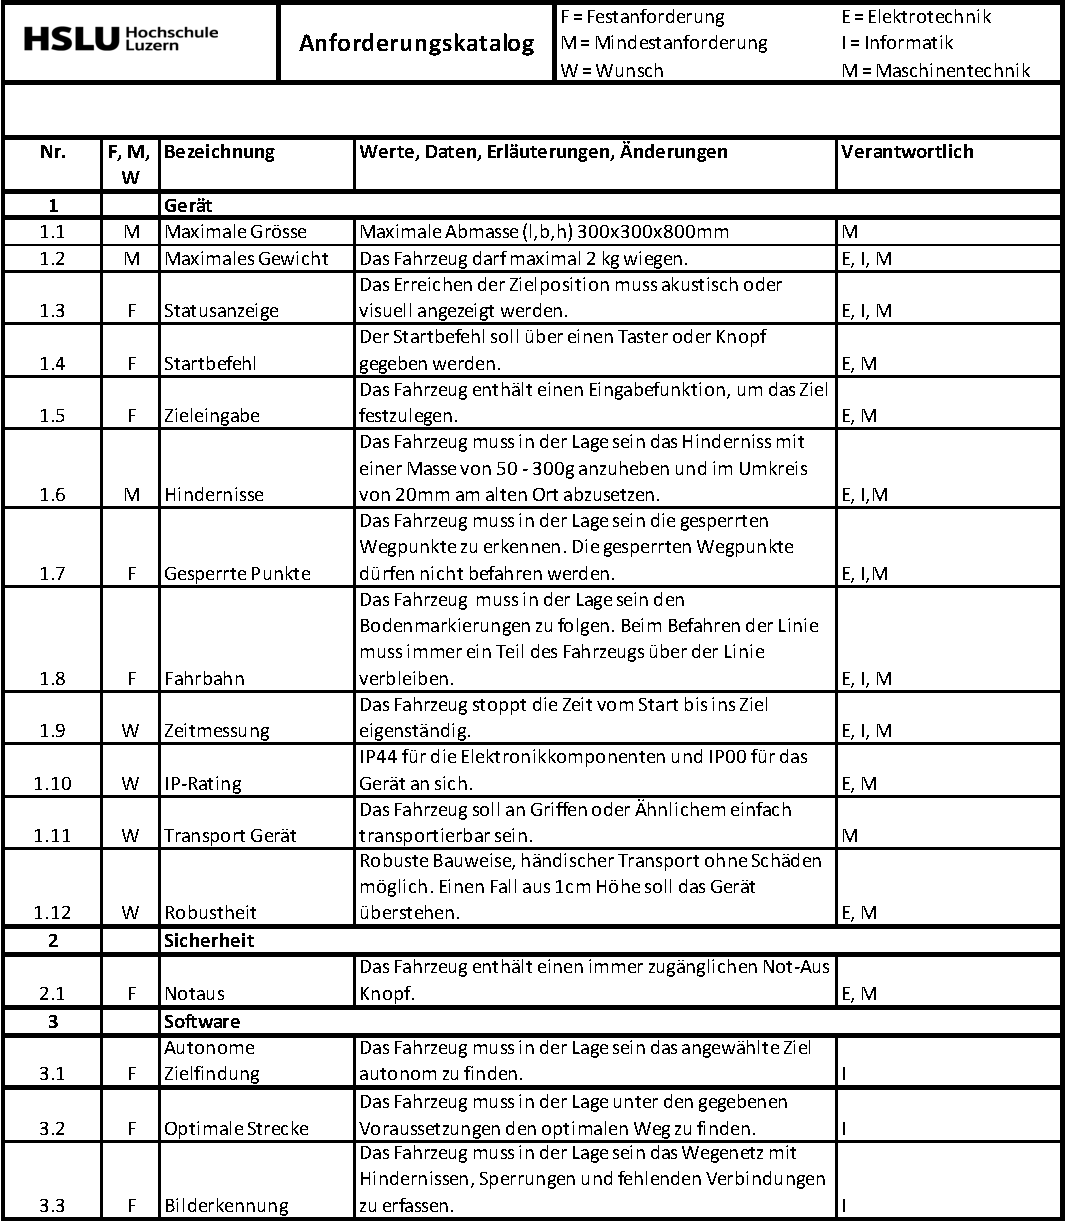
\includegraphics[width=\textwidth]{assets/projektmanagement/Anforderungsliste_V1.01_page1.pdf}
\caption{Anforderungsliste Teil 1}
\label{table:anforderungsliste_page1}
\end{table}
\newpage

\begin{table}[H]
\centering
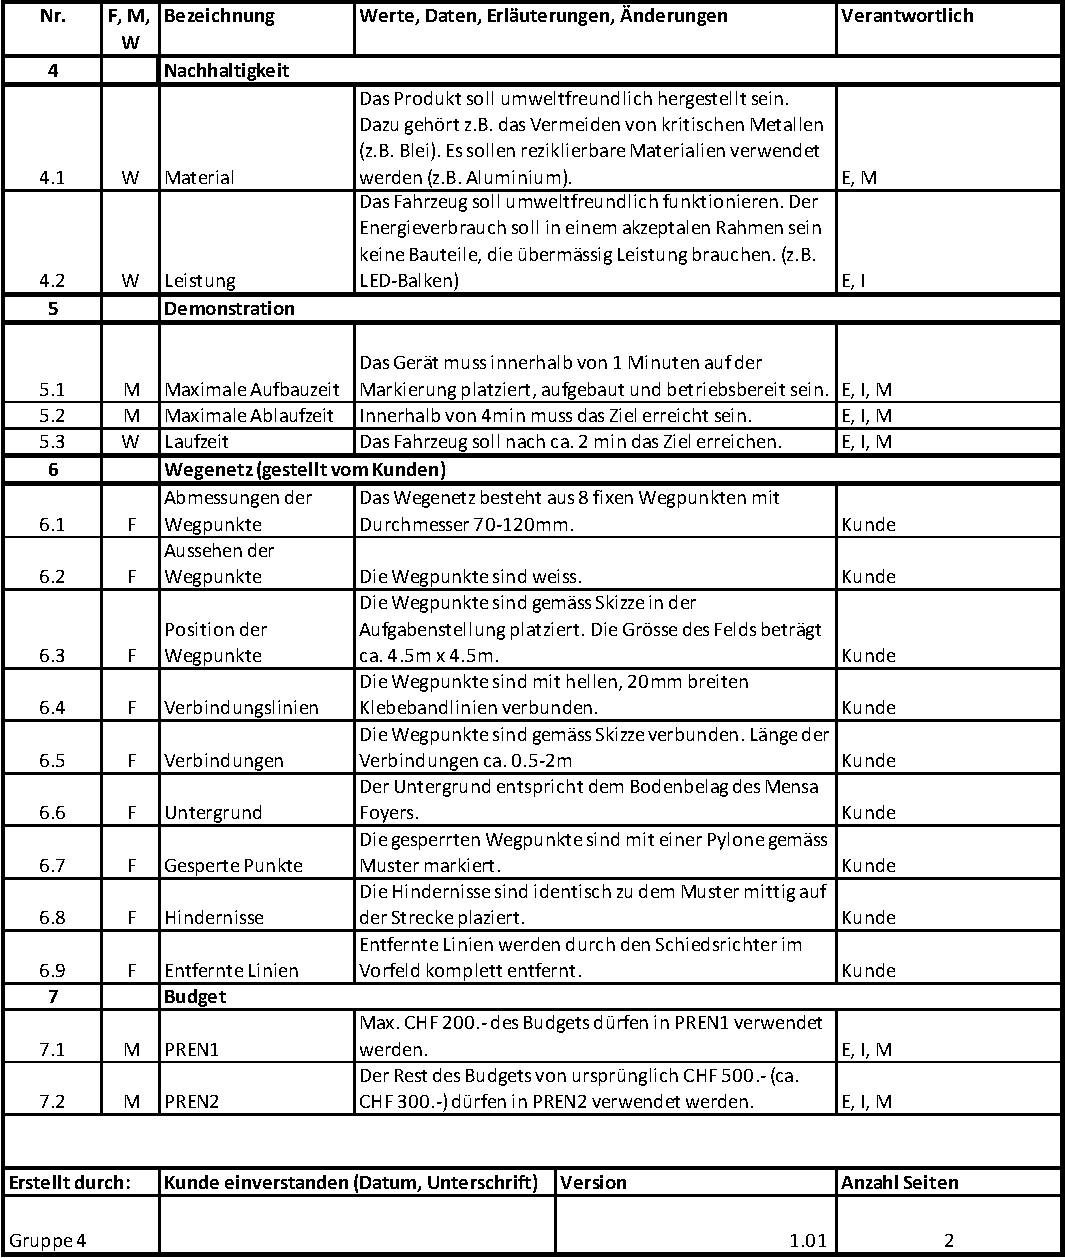
\includegraphics[width=\textwidth]{assets/projektmanagement/Anforderungsliste_V1.01_page2.pdf}
\caption{Anforderungsliste Teil 2}
\label{table:anforderungsliste_page2}
\end{table}
\newpage


%%%%%%%%%%%%%%%% Model Evaluation %%%%%%%%%%%%%%%%%%%%%%%%%5

\subsection*{YOLOv11 Model Evaluation}\label{model-evaluation}
  \addcontentsline{toc}
    {subsection}
    {YOLOv11 Model Evaluation}


TODO EXPLAIN WHAT MEANS WHAT, ADD SOURCES
TMP NOTES No sign of overfitting in 3 cols on the left (where upper row is strongly decreasing while lower row is increasing)
Training is decreasing very nicely and the lower one has some noise but overall good pattern
2 cols on the right show rapid learning and then plateauing as time goes on

Der Vergleich zwischen mehreren potentiellen Modellen ist in folgendem Dokument ersichtlich. Zwei Modelle wurden jeweils verglichen aufgrund von mehreren Werten. Ist der jeweilige Wert des einen Models besser, wird diese Zelle gruen eingefaerbt.

\includepdf[pages=-]{assets/IT/testing/yolo/ModelComparison.pdf}


%%%%%%%%%%%%%%%%%%%%%%%%%%%% Unittests %%%%%%%%%%%%%%%%%%%%%%%%%%%

\subsection*{Navigation automatisierte Unittests}\label{nav-unittests}
  \addcontentsline{toc}
    {subsection}
    {Navigation automatisierte Unittests}

TODO ADD FOR EACH MODULE THAT WE HAVE, SHOW IMAGES WHERE WE USE IMAGES